\chapter{System Model}

\section{Overview}
In the above studies, we are ready to recognize tweets sentiments and studied in case or now not have difficulty to inventory markets. Large numbers of researches which are achievable to expect different market shares, in concluding expenses with corresponding to absorption, however, those extensively passes by European markets. On account of this, we end up with the conclusions by using discussed the DJIA values. This index includes top agencies of the world market with high-quality capitalization. Even as we need to confirm which forecast is tranquility affordable in a decreasing feed of tweets, although this is wising to comfy a comparatively massive core if anyone wants to practice applying different models. Obviously, many other international customers may additionally upload their opinions in English. By international stakeholders, taking them into attention in the sentiment analysis seems valid because the DJIA value is an influent.\\

Any other essential discussion and that have the benefit to be stated in lots of works and the opportunity of sentiment lexicons online. For positive, the most certain assets are accommodated in English. Then, collecting tweets and inventory information for the diverse timelines of different conditions. We are capable of counting every trend over the timeline and we keep away from any possible effect of bias giving thanks to seasonal volatility. An extended length additionally lets for validating the consequences with a higher degree of self-assurance. The execution approving which follows the general framework arranged to confirm inside the following discern. We take a look at a day-by-day statistic of tweets in parallel to a day-by-day inventory trade statistic.\\

After identifying the sentiment for everyday supported tweets content, we have been capable of trying to match a version to go seeking out the correlation. We have tried to put emphasis on assumption checking as most studying forget this step and without difficulty taking delivery of hypotheses. But we are going to perform regressions before checking the assumptions due to the fact we are going to use them in some manner to validate fine effects with a selected model shown in figure 3.1 instead of forsaking it at the same time as it can still provide heuristically desirable predictions.\\

\begin{figure}[H]
    \centering
    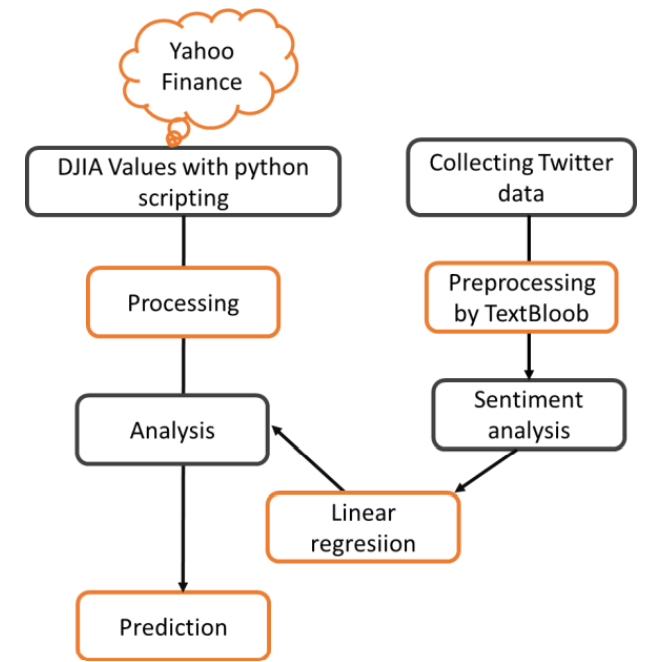
\includegraphics[scale=.7]{img3/diagram.png}
    \caption{System Model Block Diagram}
    \label{fig:Block Diagram}
\end{figure}


\section{Methodology}
While there was a lot of studies which was happened in classifying a bit of textual content as both positive or negative, there was little paintings on multi-magnificence classification. Sentiment analysis is a vital particle of our answer because this module of the output will be passed down for gaining knowledge of our predictive process. Natural language processing (NLP) is taken into consideration to be an effective device for expressing and decoding human languages like speech and textual content. Natural language processing is beneficial to textual content evaluation and textual content mining. In our experiment, we use Python and TextBlob library to perform a variety of sports related to sentiment analysis. As Python programming library has easy API, TextBlob is effortlessly able to acting primary NLP sports and tasks.\\


\section{System Design}
In this project, the system we want to evaluate the sentiment analysis tool which retrieves, processes and tests twitter data. The main purpose of our project to build a co-relation between stock prices and the overall people sentiment. At the very first step we have collected stock values from Yahoo Finance for a defined time range for our project. Next step, we have tried to collect the twitter trending data using twitter API at the same time range. Then we have pre- processed data we got from twitter and DJIA values. With textblob and python data-frame for featuring twitter data for analyzing sentiment. At the final step there is involved a linear regression algorithm for visualizing of data along with required tests.the full process is shown as a system architecture in figure 3.2. \\

\begin{figure}[h]
    \centering
    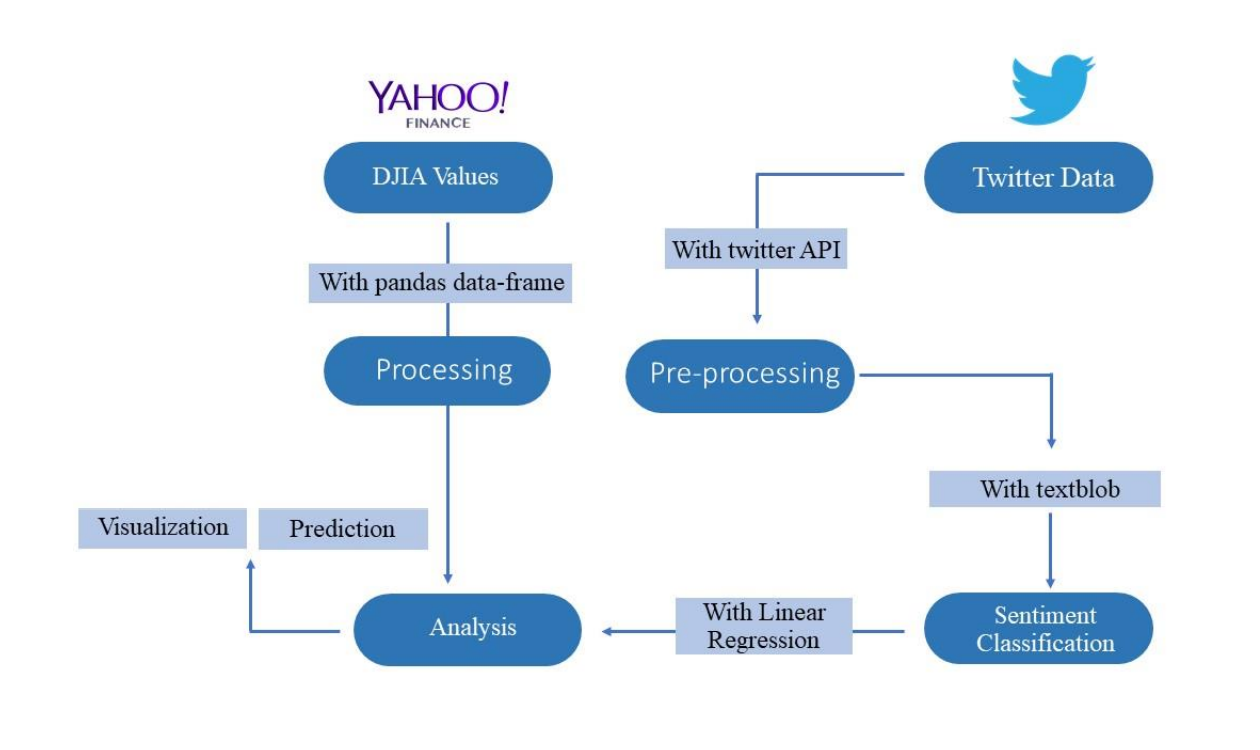
\includegraphics[scale=.6]{img3/System Architecture.png}
    \caption{System Architecture}
    \label{fig:System Architecture}
\end{figure}


\section{Data Set and Preprocessing}
Because the ways of data collection can get in large portions, it has become difficult to identify from which source we extract data or exactly which messages are selected for doing sentiment analysis. Raw inventory price statistics are pre-processed before inputting into machine getting to know various models. Pre-processing consists of reworking the uncooked records within a layout which process can take from and function on, most possibly characteristic matrix. It allows extracting some features, monetary-area-particular especially, manually to enhance outcomes, allowing the model to research greater abstractions. The data we have collected for this research is mainly from 2020 till now.\\

In our study, we’ve collected random twitter data by using Twitter API, which we applied for. For the need of our experiments, we’ve collected random Twitter posts of that point as numeric data. These numeric data associated with finances are collected from Yahoo! Finance website. The latter is that the property of Yahoo! was founded to supply economic and financial news and commentary covering share prices, financial press releases, financial reports, etc. We collect each data while aggregating numeric data supported attributes of share prices with opening, high, low and shutting rates (OHLC). This data set is critical because it is employed to support predictive analyses on the future movement of share prices.The dataset processing is illustrated in figure 3.3. \\


\begin{figure}[H]
    \centering
    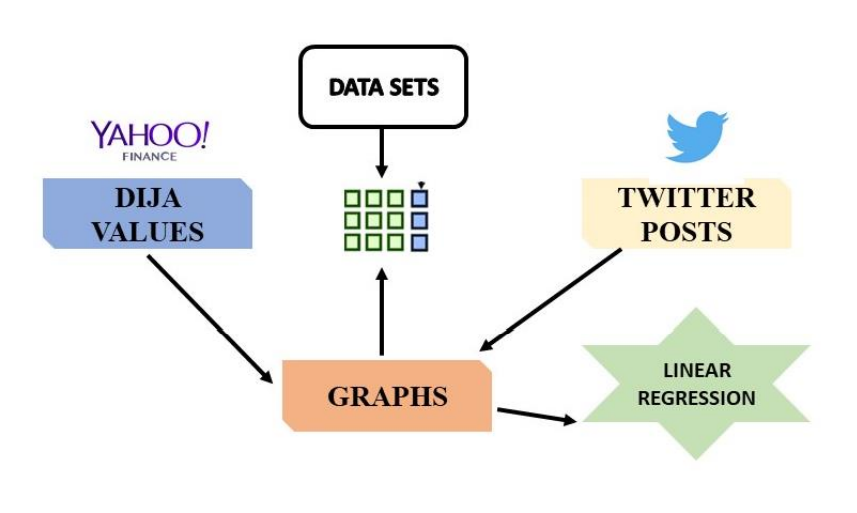
\includegraphics[scale=.65]{img3/Dataset Pre-processing.png}
    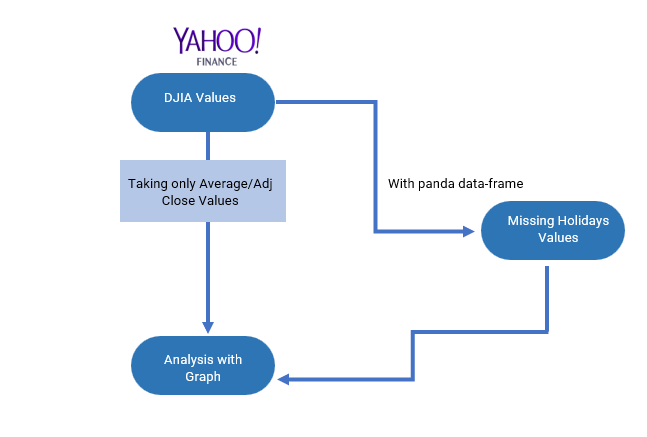
\includegraphics[scale=.9]{img3/Dataset Pre-processing2.png}
    \caption{Dataset Pre-processing}
    \label{fig:Dataset Pre-processing}
\end{figure}


\subsection{DJIA Value}

The main dataset for this study is the inventory stock data. For example, that index-wide variety industrial common (DJIA) is taken into consideration. 
To begin, create two variables: $start\_date$ and $end\_date$. If each date founds in yfinance, then the djia-values will be downloaded as a csv file, and finally the procedure has come to an end. Here, given below in the algorithm 1 which is used to extract DJIA data.\\

\begin{algorithm}
\caption{DJIA Data Extract}\label{alg:djia}
\begin{algorithmic}[1]
\State $each\_date \gets (start\_date, end\_date)$
\State $stock \gets 'dji'$
\For{$each\_date \in stock$}
    \If{$start\_date \leq end\_date$}
        \State $djia\_values \gets yfinance.download(stock,each\_date)$
    \EndIf
\EndFor
\State $djia\_data \gets pandas.dataframe(djia\_values)$
\\\textbf{Return}
\textit{djia\_data}
\end{algorithmic}
\end{algorithm}

The primary information for the stock price records became to be had on the Yahoo finance website. The know-how became accrued by writing a python script to carry out internet scraping.\\

\begin{figure}[H]
    \centering
    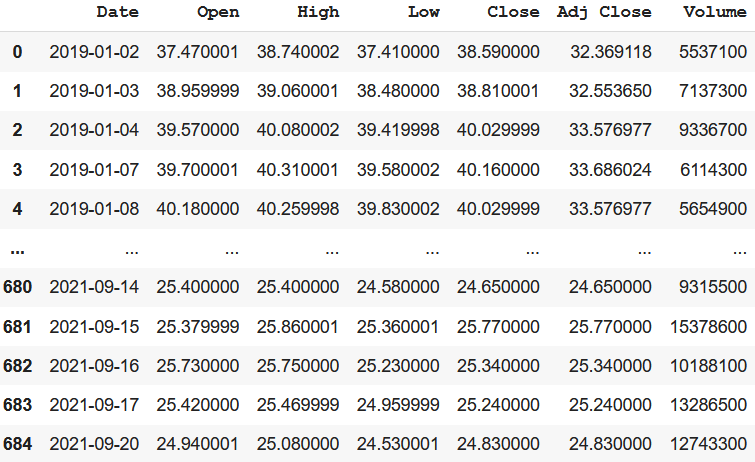
\includegraphics[scale=.8]{img3/Collected DJIA Values.png}
    \caption{Collected DJIA Values}
    \label{fig:DJIA Values}
\end{figure}

Through this net scraping shown in figure 3.4, the statistics are accumulated and stored as a comma-separated value (CSV) record. It’s to be cited right here that most effective the inter-day buying and selling values are acquired. This refers back to the trading performed across diverse days and intra-day refers to the trade carried out in the day. This can be because the intraday trading fees don’t appear to be readily available similar to the inter-day expenses and it also will increase the computational need and complexity. An additional piece of key statistics that may not be acquired is the order e-book. It can help provide a prediction of the rate using the weighted average of the orders.\\



\subsection{Twitter Data}
Tweets are on hand via a truthful seek of requisite phrases via a utility programming interface (API). Currently, over 500 million messages are published on Twitter on an everyday foundation as we can see in figure 3.5. This takes a look at turned into carried out over a length of eight months length that is already instructed in the introduction. During this era, we’re amassing English tweets wherein every tweet file contains various identifiers, languages, texts and different submitted dates/times to reach as we have directed our goal on trending tweets wherein tweets are different quite trades and mentioned generation stocks which have excessive tweet versions. \cite{bhardwaj2015sentiment}\\
\begin{figure}[H]
    \centering
    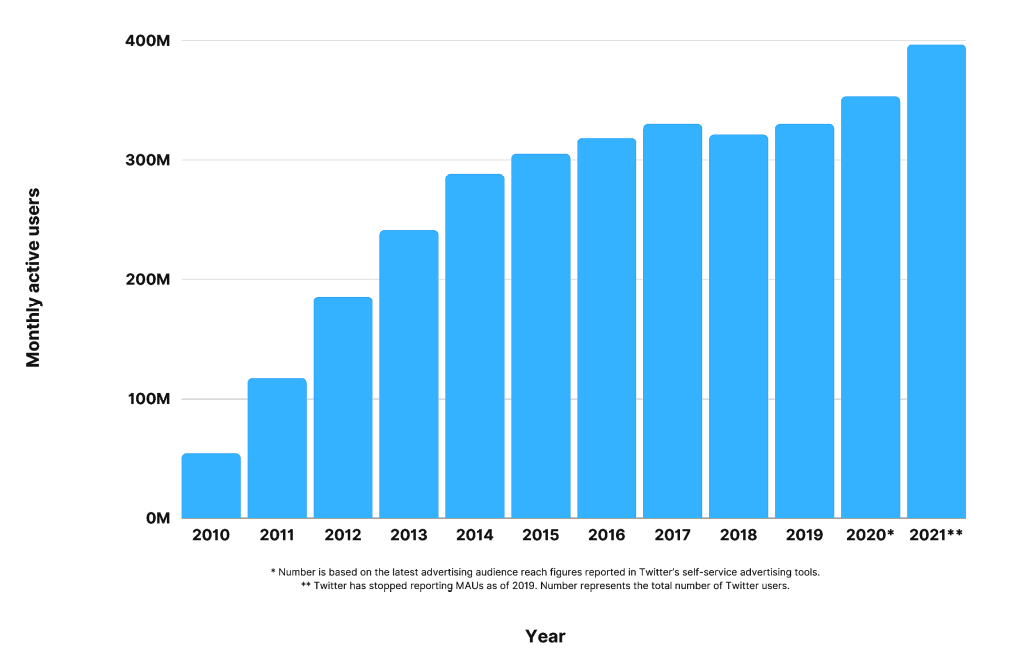
\includegraphics[scale=.5]{img3/Twitter Users.png}
    \caption{Twitter Users Growth}
    \label{fig:Twitter Users}
\end{figure}

While the Twitter statistics became to be had for all day mendacity withinside the given timeline, the DJIA values are required the usage of Yahoo! Finance website became missing data for weekends and different desertions while that marketplace is shut. To finish these statistics, we resembled those lacking ethics the usage of pandas data-frame work.\cite{noauthor_count_2020}\\

In the following steps how to obtain twitter API keys:
\begin{itemize}
    \item[--] Login to twitter developer section.
    \item[--] Go to “Create an App”.
    \item[--] Fill the details of the application.
    \item[--] Click on Create your Twitter Application
    \item[--] Details of your new app will be shown along with consumer key and consumer secret.
    \item[--] For access token, click” Create my access token”. The page will refresh and generate access token.
\end{itemize}
    
After getting twitter API, we try to collect and extract twitter data. In given below algorithm which is used to help collecting and extracting twitter data.\\

To extract data from Twitter, we'll need the API keys, which will allow us to start collecting data.We gained access to many keys after gaining access to the Twitter API.We use the following keys for data extraction: customer key, customer secret key, access key, access secret key, and access token key.We fixed these keys after initializing them as variables because they differed from user to user.We can get the author of any tweet using this API, which we use below with trending tweets available at different periods.Then, to get the available trending tweets on a specific day, we create a condition and put them into a try loop. If it doesn't work, we'll double-check the keys we received as well as our network connection.Then, in our trending data, we search for trending terms and select the most popular ones to create raw data, which we use to initialize for api search, q=word, and get the results of popular tweets.Finally, we save the tweet data as raw data for our collection using Pandas Frame.The algorithm 2 below, which is used to collect and extract Twitter data, is as follows:\\

\begin{algorithm}[H]
\caption{Twitter Data Extract and Collect}\label{alg:tweet}
\begin{algorithmic}[1]
\Require API Keys
\State $tweet\_data \gets variable to collect tweet data$
\State $consumer\_key \gets tweet api customer key$
\State $consumer\_secret \gets tweet api customer secrect key$
\State $access\_key \gets tweet api customer acess key$
\State $access\_secret \gets tweet api customer secret acess key$
\\\textbf{try}
    \State $\indent auth \gets tweepy.OAuthHandler(consumer\_key, consumer\_secret)$
    \State $\indent auth.set\_access\_token(access\_key, access\_secret)$
    \State $\indent api \gets tweepy.API(auth)$
    \State $\indent print('Authorized!')$
\\\textbf{except}
    \State $\indent print('Error!')$\\
    
\State $raw\_data \gets []$
\State $trending\_data \gets api.trends\_place(id=1)$
\For{$trending\_word \in trending\_data$}
    \For{$word \in trending\_word['trends']$}
        \State $raw\_data \gets tweepy.Cursor(api.search,q=word,type='popular')$
    \EndFor
\EndFor
\State $tweet\_data \gets pandas.dataframe(raw\_data)$
\\\textbf{Return}
\textit{tweet\_data}
\end{algorithmic}
\end{algorithm}


\section{Sentiment Analysis}
To categorize given contextual content in order to map it to elegance, sentiment analysis is used. Sentiment Analysis may be binary, i.e., high-quality or negative or multi-elegance with three or extra instructions involved. The sort of sentiment evaluation relies upon on dataset and reasoning method adopted. Researchers and stakeholders frequently diverge on their interpretation of courting that exists among sentiment evaluation and detection of emotion. While their factors of view may also fluctuate primarily based totally on their respective perspectives, researchers are united in adopting similar techniques. It is a manner to gauge or decide the emotion of the writer. The emotion can either be nice, bad or neutral. TextBlob’s sentiment characteristic evaluates to 2 properties polarity and subjectivity. Subjectivity belongings values also are flow that falls inside the variety of [0, 1]. How we have worked on our project with text blob are shown in the following figure 3.6:\\

\begin{figure}[H]
    \centering
    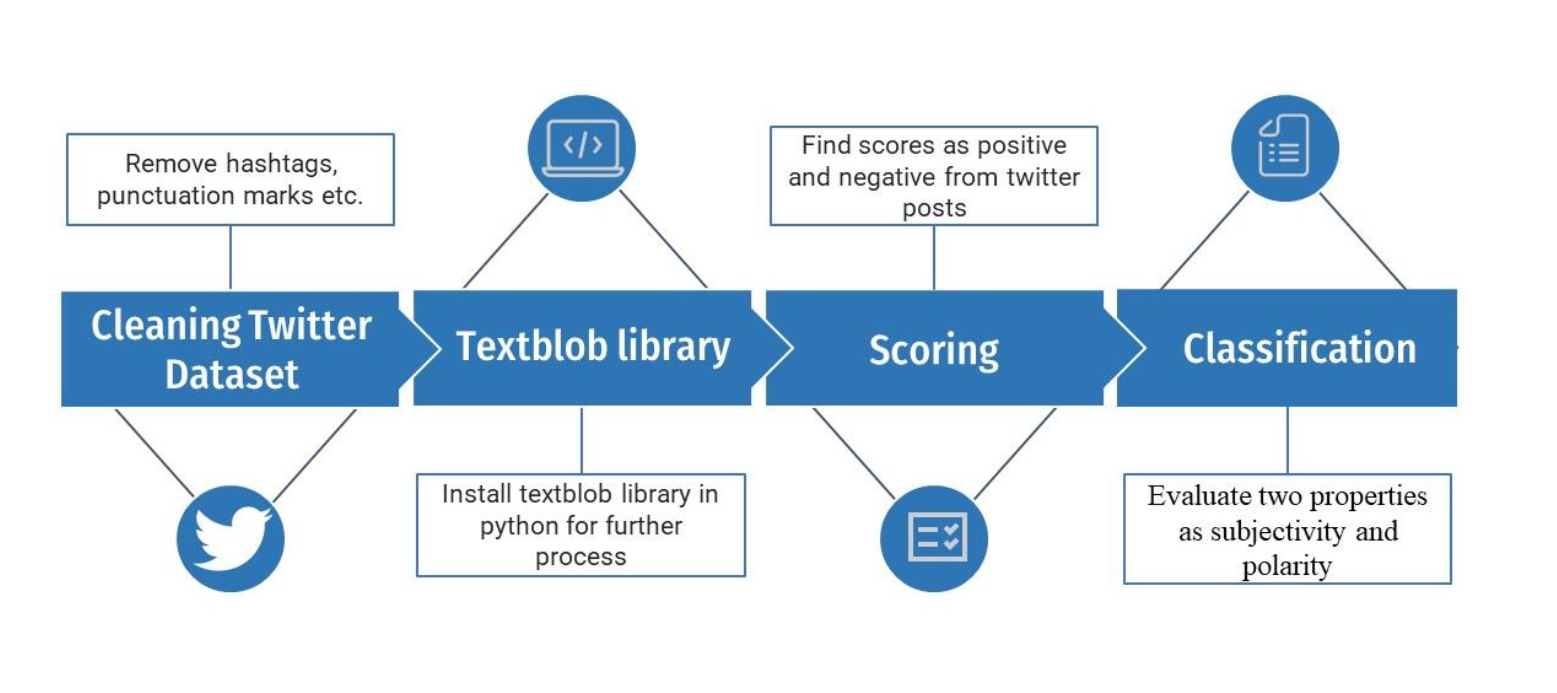
\includegraphics[scale=.45]{img3/Textblob Working Process.png}
    \caption{Textblob Working Process}
    \label{fig:Textblob}
\end{figure}

n this study, the opinion of various peoples of various countries has been discussed. the most focus of this paper is on Twitter, Twitter API and have implemented the python artificial language and to implement the sentimental analysis as positive, negative and neutral. 
In order to make the Twitter API more relevant, we'll first import Tweepy. Then use tweet data, all tweets, tweet value, SE (set of emoji), SSC (set of special characters), SP (set of punctuations), and clean tweet as variables. Following that, we'll download tweets as datasets and save them to a CSV file. Additionally, the all-tweets variable is used to get tweets from the dataset, and the SE, SSC, and SP variables are used to remove and eliminate harmful emoji, \#tags, special characters, and punctuation from tweets. Create a new CSV file for all clean tweets. The given algorithm helps us to organize and sanitize Twitter data. \\

\begin{algorithm}
\caption{Tweet Filtering Algorithm}\label{alg:Filter}
\begin{algorithmic}[1]
\Require $tweet\_data$
\State $temoji \gets set of Emojis$
\State $schar \gets set of special characters$
\State $punc \gets set of punctuations$
\\
\State $raw\_tweets \gets tweet\_data$
\For{$tweet \in raw\_tweet$}
    \If{$emoji = schar = punc \not= [NULL]$}
        \State $clean\_tweet \gets remove \in emoji, schar, punc$
    \EndIf
\EndFor
\State $clean\_data \gets pandas.dataframe(clean\_tweet)$
\\\textbf{Return}
\textit{clean\_data}
\end{algorithmic}
\end{algorithm}



We’ll tokenize every phrase withinside the dataset and keep it into the dataset. for each phrase, will evaluate it with positive, terrible and impartial sentiments phrase withinside the dictionary. Then increment the positive, terrible and impartial count. Finally, based totally on the positive, terrible and impartial count, we are ready to get the top result percent approximately sentiment to see the polarity. this study suggests the sentimental evaluation set of rules at an excessive level. As may be visible withinside the algorithm 3, researchers have distinct approaches to attach the Twitter API, four fetch the tweets, tweet cleansing or do away with preventing phrases and punctuation marks, classify tweets because of this that get the polarity of the tweet, and finally go back the results. In this paper, python is used to put in force the sentimental evaluation. Some applications have been applied along with tweepy and textblob.[6] \cite{mittal2012stock} The required 
libraries are mounted with the aid of using following commands:\\
$\blacktriangleright$ pip set up tweepy\\$\blacktriangleright$ pip set up textblob\\

The main steps of this sentiment analysis are drawn in following figure 3.7:\\

\begin{figure}[H]
    \centering
    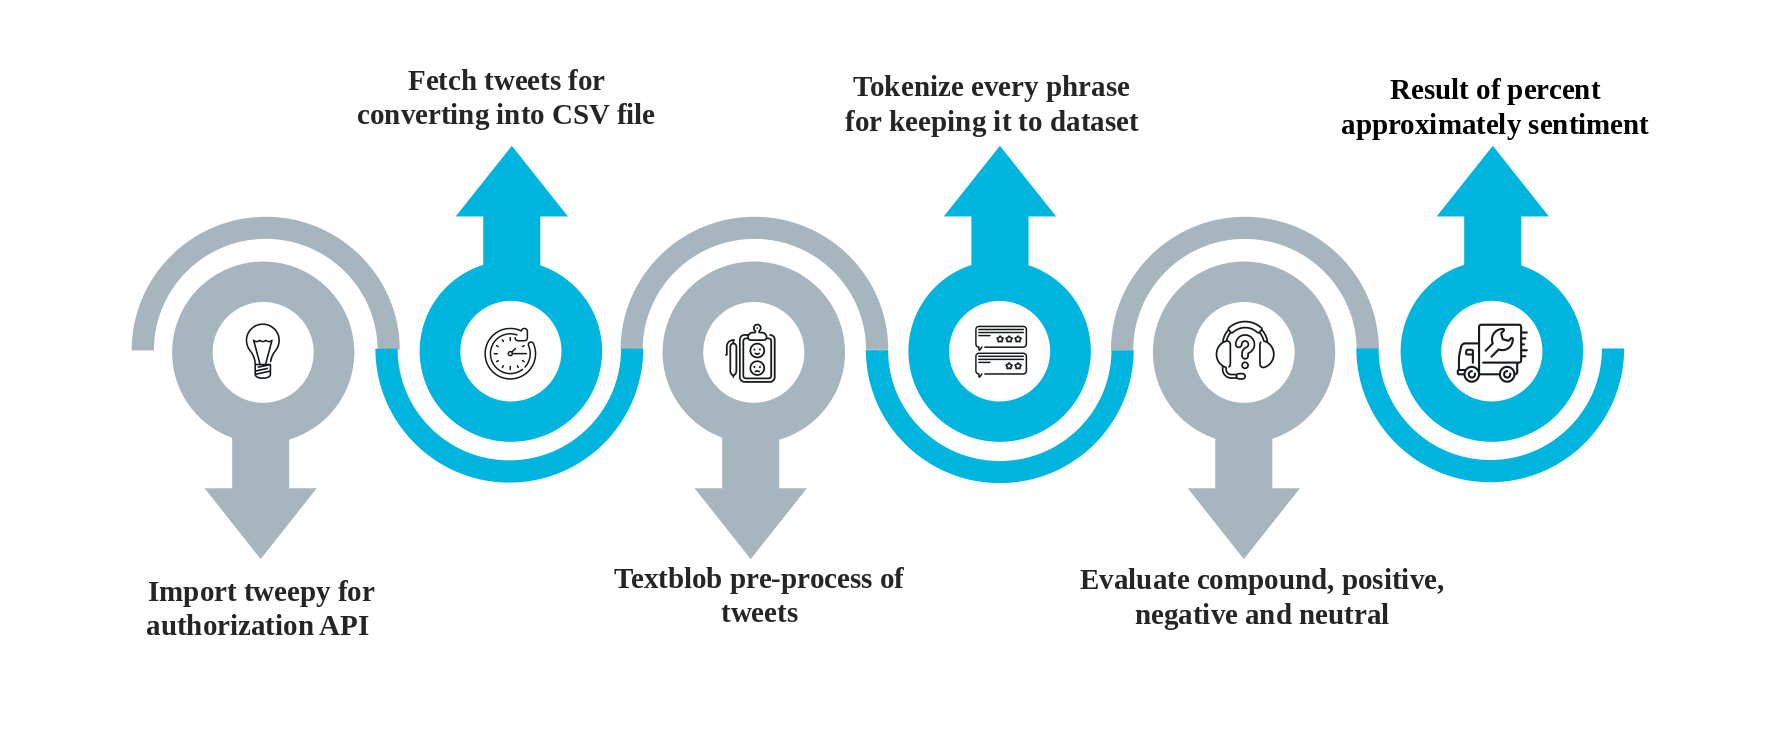
\includegraphics[scale=.3]{img3/Sentiment Analysis Process.png}
    \caption{Sentiment Analysis Process}
    \label{fig:Sentiment Analysis}
\end{figure}


\section{Hypothesis and Final Co-relation}
For getting better result and prediction, we at first find out the p-value of our twitter data. We applied this co-efficient so that we can know whether the prediction of our data will be possible to get or not. A probability associated with a crucial value is known as a p-value. The crucial value is determined by the possibility of a Type mistake being allowed. It calculates the probability of achieving results that are as least as good as if the claim (H0) were true.\\

A correlation matrix is a table that displays the coefficients of correlation between variables. The correlation between two variables is shown in each cell of the table. A correlation matrix can be used to summarize data, as an input to a more sophisticated study, or as a diagnostic tool for advanced analyses.The instances in a predicted class are represented by the rows of the matrix, whereas the instances in an actual class are represented by the columns (or vice versa). The name is derived from the fact that it is simple to observe if the system is mixing up two classes (i.e. commonly mislabeling one as another). It's a unique type of contingency table with two dimensions ("polarity" and "subjectivity") with identical sets of "classes" in each dimension. As we know if p-value is stayed at between 0 to 0.1 it is possible to make prediction on that dataset. After applying p-value we got the average result 0.06, 0,07 and 0.3. We know the range of p value is -1 to 1. Since our result is 0.06,0.07,0.3 so, ours dataset is ready for working . The p-value correlation coefficient of our dataset is given below in figure 3.8: \\

\begin{figure}[H]
    \centering
    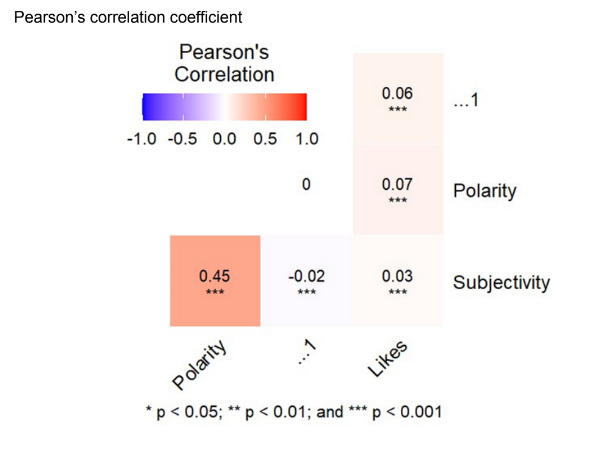
\includegraphics[scale=.9]{img3/Pearson.png}
    \caption{Pearson’s correlation coefficient}
    \label{fig:Pearson’s correlation coefficient}
\end{figure}

This study will try to show the following hypothesis in order to analyze the market.\\
H1: The total averaged sentiment of all stocks within a sector will be used to determine the
sentiment of the sector.\\
By using people sentiment, we will be able to identify their positive, negative thinking and whether their thinking is affecting a particular sector or not. The result of this hypothesis is clearly shown and explained in our result section with appropriate values and graph.\\\\
H2: On any given day, the sentiment of a sector or stock will provide a forecast for that stock’s
movement the next day.\\
We will know if the stock price will be up or down the next day or next moment of any day. By using this hypothesis, it will be easier for making any decisions to invest at their will. The overall prediction and accuracy level have been compared with our predicted values. To understand better it has been explained in detail at the result section with scatter plot by applying linear regression on our data.\\\\
H3: The stocks with the highest number of Twitter mentions are also the stocks that lend the
most weight to a sector’s mood.\\
From this thinking, we can know which type of sentiments are actually making effect on stock prices. The sentiments of tweet will be clearly shown with related graph and values to understand. We will work on more data so that we can understand people’s mood who are directly investing on share market. To know their mood, we need more data and also need to do real time survey on those people which will be time consuming so far for which we will work in future on that.\\

\section{Linear Regression (Proposed Algorithm)}
The linear regression set of rules tries to research a characteristic that maps enter vectors to scores. It represents with the aid of using a linear mixture of the enter capabilities. We will try to use an ahead step-clever technique to set the mass in order to carry out the characteristic collection. At the very early stage, we have to fix the implied evaluation rating. After this, till the favored variety of entering capabilities were delivered, enter capabilities have been delivered differentially. At every stride, that characteristic which will minimize corrupted mistakes maximum when delivered became collected. If the time of delivering, its mass fixes as if corrupted mistakes could be reduced, then given that capabilities and mass already delivered. That variety to enter capabilities consisting of became decided with the aid of using validation \cite{bhardwaj2015sentiment}. The working process of this algorithm is drawn at step by step in the following figure 3.9:
\begin{figure}[H]
    \centering
    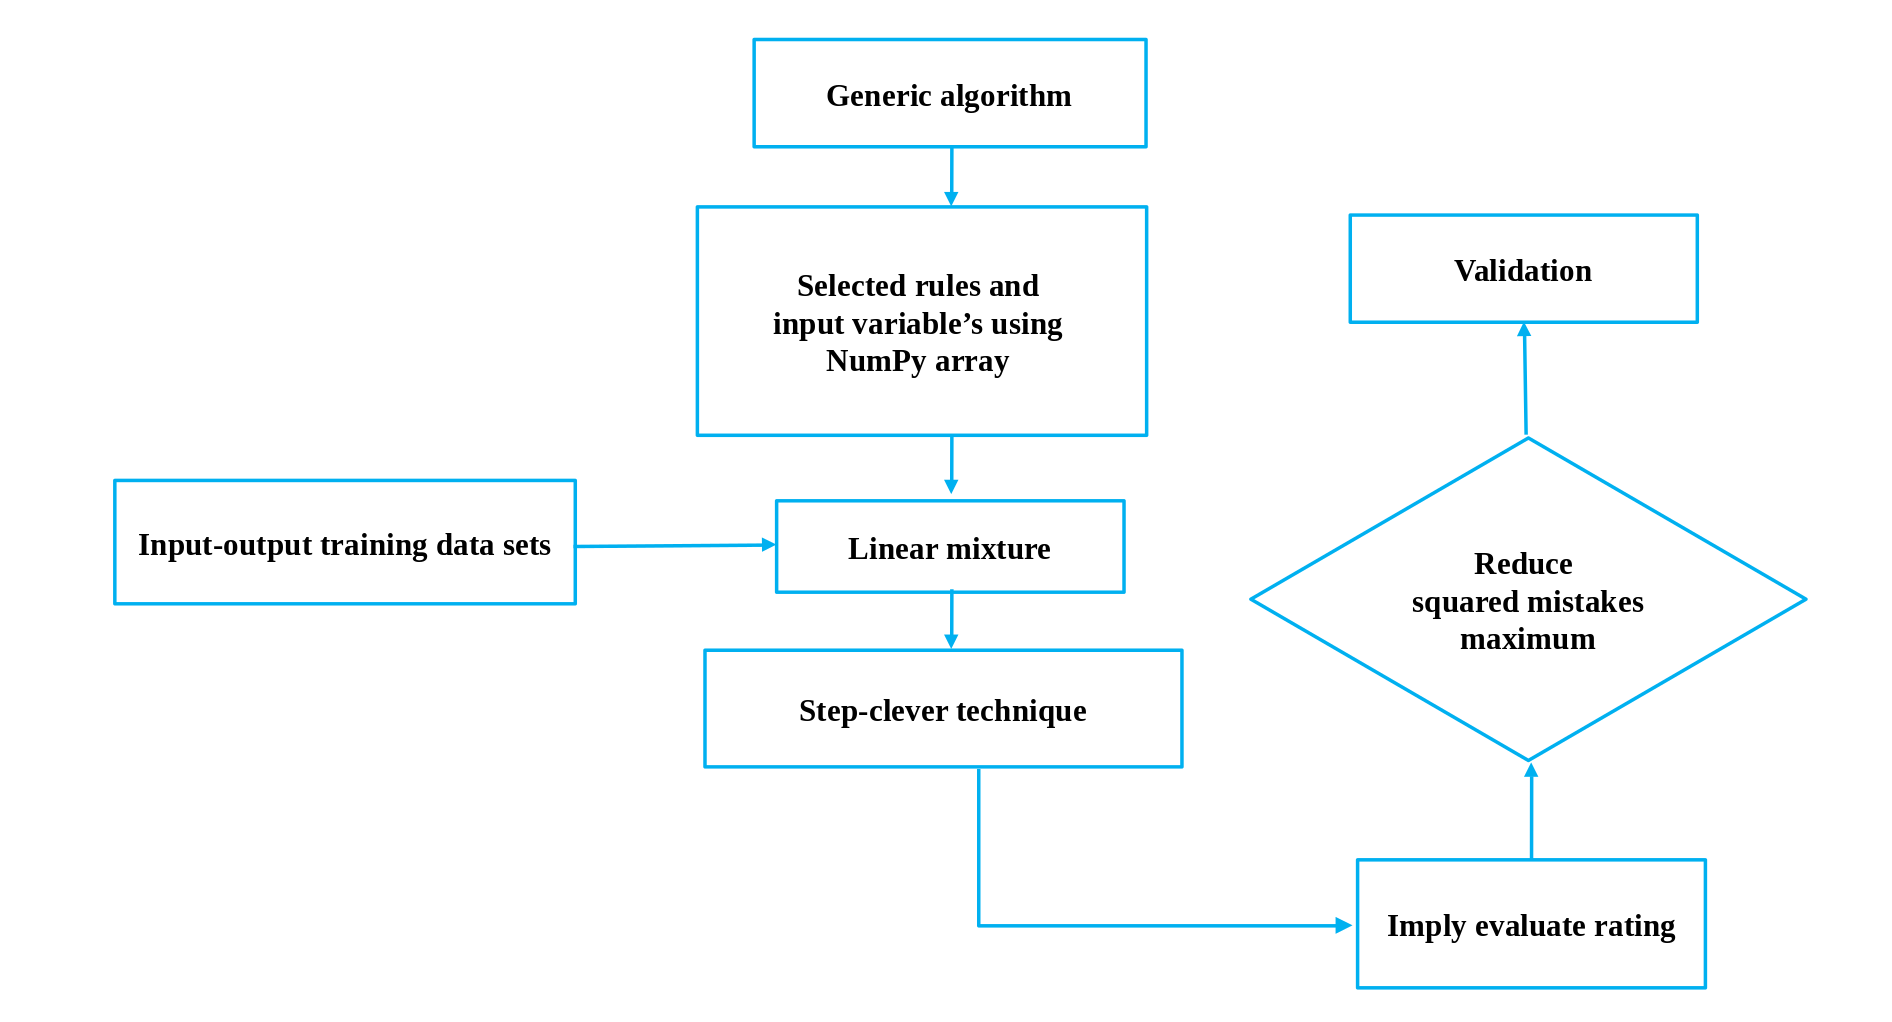
\includegraphics[scale=.3]{img3/Linear Regression Workflow.png}
    \caption{Linear Regression Workflow}
    \label{fig:LR Workflow}
\end{figure}
